\section{What disclosure buys}\label{sec:disclosure}

Because active probing is costly and passive data are slow, the natural policy question is what a supervisor gains from disclosure. We compare six observation contracts at $\delta=0.05$.
\begin{itemize}[itemsep=1pt]
\item $I_0$: public prices only.
\item $I_1$: prices and aggregated executed flow.
\item $I_2$: prices and one independent noisy report of dealer marked equity per reset ($\sigma_E=0.5$).
\item $I_3$: prices and exact audited equity (Proposition~\ref{prop:disclosure}), also with reports rounded to $0.01$.
\item $I_4$: algorithm update timestamps without the update values.
\item $I_5$: a supervisory audit registry with access to internal algorithm states.
\end{itemize}

\begin{table}[t]\centering\small
\begin{threeparttable}
\caption{Disclosure contracts at $\delta=0.05$ (pulse-design capital, par units)}\label{tab:contracts}
\begin{tabular}{llrrr}
\toprule
Contract & Channel & Pulses & Benchmark & Saving vs.\ $T=20$\\
\midrule
$I_0$: prices, $T=3$ & public prices & 271 & 4{,}305.25 & $-2{,}123.5\%$\\
$I_0^*$: prices, $T=20$ & full price path & 12 & 193.62 & 0.0\%\\
$I_1$: prices and signed flow & public flow & 12 & 193.62 & 0.0\%\\
$I_2$: noisy equity ($\sigma_E=0.5$) & statement & 12 & 193.62 & 0.0\%\\
$I_3$: exact equity, 5-unit lot & audited equity & 1 & 12.70 & 93.4\%\\
$I_3$: exact equity, 0.01 rounding & rounded report & 1 & 15.52 & 92.0\%\\
$I_4$: timestamps only & no likelihood & 12 & 193.62 & 0.0\%\\
$I_5$: audit registry & internal states & 0 & 0.00 & 100.0\%\\
\bottomrule
\end{tabular}
\begin{tablenotes}\footnotesize\item Closed-form values. Noisy equity adds information linearly in the number of resets, $\KL=N\Delta_E^2/(2\sigma_E^2)$, and saves only 1.5\% against the $T=3$ baseline. The equity difference is $\Delta E=\kappa^2q\delta^2V^2$; with reports rounded to $0.01$, a guaranteed change needs $V\ge5.59$.\end{tablenotes}
\end{threeparttable}
\end{table}

Table~\ref{tab:contracts} shows that disclosure is not one thing. Timestamps without update values carry no information about $\delta$ in this model. Noisy periodic statements barely help. Exact audited equity collapses the requirement to a single trade, limited only by lot sizes and report precision, and an audit registry removes the trading requirement altogether.

The cleanest form of useful disclosure is flow tagged by participant class.

\begin{proposition}[Tagged flow removes the barrier]\label{prop:tagged}
Let the price be driven by i.i.d.\ innovations of variance $\sigma_\xi^2$ in a positive, stable economy, with stationary autocovariances $\gamma_x(s)=\sum_\ell c_\ell\lambda_\ell^{|s|}$ ($c_\ell\ge0$, $0\le\lambda_\ell<1$ the closed-loop modes). Suppose cohort $i$ has merged weight $w_i>0$ and the observer receives prices and each cohort's flow $\tilde u_{i,t}=u_{i,t}+\varepsilon_{i,t}$, $u_{i,t}=q_iy_{i,t}$, with i.i.d.\ measurement noise of variance $\sigma_f^2$ independent of prices. Then $\tilde u_{i,t}=r_i\tilde u_{i,t-1}+w_ix_t+e_{i,t}$ with $e_{i,t}=\varepsilon_{i,t}-r_i\varepsilon_{i,t-1}$, and the just-identified IV estimator of $\beta_i=(r_i,w_i)$ with instruments $Z_t=(x_{t-1},x_t)^\top$ satisfies $\sqrt T(\hat\beta_i-\beta_i)\to N(0,V_i)$,
\begin{equation}\label{eq:ivvar}
V_i=\Sigma_i^{-1}\Omega_i\Sigma_i^{-\top},\qquad \Sigma_i=\begin{pmatrix}w_iA_0&\gamma_x(1)\\ w_iA_1&\gamma_x(0)\end{pmatrix},\qquad \Omega_i=\sigma_f^2\bigl[(1+r_i^2)\Gamma_0-r_i(\Gamma_1+\Gamma_1^\top)\bigr],
\end{equation}
where $A_m=\sum_{s\ge0}r_i^s\gamma_x(s+m)$, $\Gamma_0=\begin{psmallmatrix}\gamma_x(0)&\gamma_x(1)\\ \gamma_x(1)&\gamma_x(0)\end{psmallmatrix}$ and $\Gamma_1=\E[Z_tZ_{t-1}^\top]$. The Jacobian determinant is
\begin{equation}\label{eq:ivdet}
\det\Sigma_i=w_i\sum_{\ell,m}c_\ell c_m\frac{1-\lambda_\ell\lambda_m}{1-r_i\lambda_m}\;>\;0 .
\end{equation}
$V_i$ depends only on cohort $i$'s own $(w_i,r_i)$, $\sigma_f^2$ and the price autocovariances, which are bounded and nondegenerate uniformly on a uniformly stable family with merged weights bounded below, whatever the rate spacing; so the merged weights are estimated at rate $T^{-1/2}$ with a constant that does not depend on $|r_i-r_j|$.
\end{proposition}

\paragraph{In words.} If each group's trading is reported separately, each group becomes an ordinary regression. Its precision depends on the group's own rate and on the price dynamics, but it has no singularity as the groups' rates approach each other.


Each tagged flow follows $u_{i,t}=r_iu_{i,t-1}+w_ix_t$, a regression whose information about $w_i$ does not involve the other cohorts' rates; the closed form \eqref{eq:ivdet} matches the simulated Jacobian ($0.1330$ against $0.1322$ in a two-cohort economy with $4\times10^5$ periods; \texttt{hardening/p1\_checks.py}). In simulation ($T=5{,}000$, 60 replications) the root-mean-square error of the recovered weights is flat in $\Delta\eta$ (fitted slope $0.011$, error between $5.8\times10^{-4}$ and $6.6\times10^{-4}$). This is the formal content of a disclosure regime such as a consolidated audit trail: tagging flow by participant class turns a polynomial barrier into an ordinary estimation problem.

\subsection{How much disclosure is worth}\label{sec:discvalue}

Proposition~\ref{prop:tagged} says that tagging removes the barrier; the next result says by how much.

\begin{theorem}[Value of class-tagged disclosure]\label{thm:discvalue}
Take a rich class of Theorem~\ref{prop:esprit}: rates $r_c+\Delta\eta\,s$ with $s$ in a compact set of $\gamma$-separated ordered points that has nonempty interior and contains the Gauss and Gauss--Radau pair of Theorem~\ref{thm:kcohort}, and merged weights in a nondegenerate interval $[\omega_{\min},\omega_{\max}]$, $0<\omega_{\min}<\omega_{\max}$. In each reset experiment the observer applies a unit impulse and records the price response with independent $N(0,\sigma^2)$ noise per tap; under tagging it also records each class's flow response $f_{i,t}=w_i\sum_{s\le t}r_i^{\,t-s}h_s$ with independent $N(0,\sigma_f^2)$ noise per tap. Let $N_p$ and $N_t$ be the numbers of experiments needed, without and with tagging, for a fixed accuracy and confidence. There are constants $0<c\le C<\infty$, depending on $(\sigma,\sigma_f)$ and the class but not on $\Delta\eta$, such that
\begin{enumerate}[label=(\roman*),itemsep=1pt]
\item to recover the weights to a fixed accuracy smaller than half the weight difference between the Gauss and Gauss--Radau economies (so that recovering the weights decides between them), $c\le N_t\le C$, so $N_p/N_t\asymp(\Delta\eta)^{-(4K-2)}$;
\item to recover the rates to accuracy $c_0\Delta\eta$, for a fixed $c_0>0$ smaller than the radius of a ball contained in the class of rescaled nodes (so that no fixed guess meets the target), $c(\Delta\eta)^{-2}\le N_t\le C(\Delta\eta)^{-2}$, so $N_p/N_t\asymp(\Delta\eta)^{-(4K-4)}$.
\end{enumerate}
\end{theorem}

\begin{proof}
$N_p\asymp\sigma^2(\Delta\eta)^{-(4K-2)}$ by Theorems~\ref{thm:kcohort} and~\ref{prop:esprit}. \emph{Upper bounds.} Average the $N$ price responses to estimate $h$ with error of order $\sigma N^{-1/2}$ per tap. Given $h$, class $i$'s mean flow is a two-parameter family $F(w_i,r_i;h)$ whose Jacobian columns $\sum_sr_i^{t-s}h_s$ and $w_i\sum_s(t-s)r_i^{t-s-1}h_s$ are linearly independent, with a Gram determinant bounded below uniformly on the class because $w_i\ge\omega_{\min}$, the rates lie in a compact subset of $(0,1)$ and $h_0=\kappa>0$; the bound does not involve the other classes or $\Delta\eta$. Least squares on class $i$'s flows with the plug-in $h$ therefore estimates $(w_i,r_i)$ with error $O_P(N^{-1/2})$, uniformly on the class, which gives the upper bounds in (i) and in (ii) for accuracy $\epsilon\Delta\eta$. For (i) there is also a finite-sample version: in the first period the tagged flow of class $i$ is $w_i\kappa$, so the mean of the $N$ first-period records gives $P(|\hat w_i-w_i|\ge\epsilon)\le\sigma_f^2/(N\kappa^2\epsilon^2)$ by Chebyshev's inequality, for every configuration (this step is machine-checked). \emph{Lower bounds.} At a configuration in the interior of the class, perturb one class's weight by $\epsilon$, or its rate by $\epsilon\Delta\eta$; for small $\epsilon$ both perturbed configurations remain in the class because the weight interval is nondegenerate and the rate set has nonempty interior. The mean differences of both the price and the flow records are of order $\epsilon$, respectively $\epsilon\Delta\eta$, so the Kullback--Leibler divergence of $N$ experiments is at most $CN\epsilon^2$, respectively $CN\epsilon^2(\Delta\eta)^2$, and Le Cam's two-point lemma gives the lower bounds.
\end{proof}

\paragraph{In words.} This is the value of disclosure measured in data. Tagging replaces a requirement that explodes as the groups become similar with one that does not grow at all (for the weights) or grows only like $(\Delta\eta)^{-2}$ (for the rates).


Proposition~\ref{prop:tagged} and Theorem~\ref{thm:discvalue} use different observation arrangements: the proposition concerns passive, stationary data with prices observed without noise, where the price is a valid instrument; the theorem concerns reset experiments with noisy prices. With noisy prices, regressing flow on the observed price is an errors-in-variables problem, which is why the theorem works from the known impulse instead.

\begin{proposition}[Robustness to strategic evasion: Sybil splitting, camouflage, and chilling]\label{prop:strategic}
Consider the class-tagged disclosure regime of Theorem~\ref{thm:discvalue} and Proposition~\ref{prop:tagged}. Let trader group $i$ attempt to evade supervisory identification through one of three strategic responses:
\begin{enumerate}[label=(\roman*)]
\item \emph{Sybil account-splitting.} Suppose group $i$ divides its trading volume across $M_i \ge 1$ distinct pseudonymous accounts or sub-entities, each executing a fraction $\alpha_{i,m} > 0$ ($\sum_{m=1}^{M_i} \alpha_{i,m} = 1$) with the same underlying memory rate $r_i$ and flow $u_{i,m,t} = \alpha_{i,m} u_{i,t} + \varepsilon_{i,m,t}$, where $\varepsilon_{i,m,t}$ is i.i.d.\ reporting noise with variance $\sigma_{f,m}^2$. Then for each sub-account $m$, the instrumental-variables Jacobian determinant satisfies
\begin{equation}\label{eq:sybil_det}
\det \Sigma_{i,m} = \alpha_{i,m} w_i \sum_{\ell,k} c_\ell c_k \frac{1-\lambda_\ell \lambda_k}{1-r_i\lambda_k} > 0,
\end{equation}
which is bounded strictly away from zero for any non-vanishing sub-account ($\alpha_{i,m} \ge \underline{\alpha} > 0$). Group $i$'s total weight $w_i = \sum_{m=1}^{M_i} \hat w_{i,m}$ and common persistence rate $r_i$ are identified at the standard parametric rate $T^{-1/2}$, with no polynomial degradation in $\Delta\eta$.
\item \emph{Strategic camouflage and noise injection.} Suppose group $i$ injects uninformative pseudo-random trading noise $\zeta_{i,t}$ with variance $\sigma_{\zeta}^2$ into its orders to obscure its regression signature. To lower the signal-to-noise ratio sufficiently to restore the price-only super-resolution complexity $(\Delta\eta)^{-(4K-2)}$, group $i$ must inject noise variance satisfying
\begin{equation}\label{eq:camouflage_cost}
\sigma_\zeta^2 = \Omega\bigl((\Delta\eta)^{-(4K-2)}\bigr).
\end{equation}
By Lemma~\ref{lem:toeplitz}, trading this camouflage volume against a linear order book incurs a cumulative per-period quadratic execution loss of at least $\frac{1}{2}\kappa \sigma_\zeta^2 = \Omega((\Delta\eta)^{-(4K-2)})$, which strictly dominates any finite expected trading profit $\Pi_i < \infty$, rendering strategic camouflage economically unviable.
\item \emph{Intensity chilling.} If group $i$ strategically curtails its trading intensity by scaling $w_i$ down to $\gamma_i w_i$ with $\gamma_i \in [\underline{\gamma}, 1]$ for some $\underline{\gamma} > 0$, the instrumental Jacobian determinant \eqref{eq:sybil_det} scales proportionally by $\gamma_i \ge \underline{\gamma} > 0$, preserving $T^{-1/2}$ identification. If group $i$ chills its activity to zero ($\gamma_i \to 0$), its contribution to market instability $S$ is eliminated, achieving the supervisor's prudential objective without enforcement.
\end{enumerate}
\end{proposition}

\paragraph{In words.} A firm cannot dodge class disclosure by splitting into shell accounts, because each sub-account still obeys the same regression and their estimated weights add back up. It cannot hide behind injected noise trades, because trading enough random volume to fake the price-only barrier costs far more in execution fees than any algorithm can make. And if it chills its trading to avoid detection, it shrinks its market impact and cures the fragility problem on its own. Full proof is in Supplement~S1.

With the same noise and lags for both observers, the Cram\'er--Rao requirements give fitted slopes of $-6.08$ for prices and $-4.34$ for the ratio at $K=2$ (theory $-6$ and $-4$). Calibrated to the class memories estimated below, prices alone would need about 333 times as many days as the published class ratios to separate the top-trader and all-account memories in BTCUSDT (rates $0.9889$ and $0.9986$ per five minutes; about 6{,}000 days against 18), and about 19 times as many in ETHUSDT (rates $0.9793$ and $0.9972$). These rates come from day-demeaned regressions, which bias persistence down (Section~\ref{sec:disc_data}), so the factors are illustrative.

\subsection{Disclosure in dollars}\label{sec:disc_dollars}
\emph{This subsection is a hypothetical scale illustration of an outside prober's shadow loss, not a public cost--benefit calculation.}

Theorem~\ref{thm:discvalue} states the value of class-tagged disclosure in samples. Theorems~\ref{thm:spectral} and~\ref{thm:kcohort} let us translate that value into a flow of round-trip trading losses for an outside participant. Two adjustments make the figures exact:
\begin{enumerate}[label=(\roman*),itemsep=1pt]
\item \emph{Exact $K$-cohort moment-gap constant.} Rather than extrapolating from Cram\'er--Rao ratios, we evaluate the spectral round-trip trading loss bound of Theorem~\ref{thm:spectral},
\[
L_{\rm rt}^*(K,\Delta\eta)\;=\;\frac{4\sigma^2 z_{1-\alpha}^2}{\sup_\omega\bigl(|\Delta\hat H_{K,\Delta\eta}(e^{i\omega})|^2/g_0(\omega)\bigr)},
\]
directly for the $K$-point Gauss versus Gauss--Radau economies of Theorem~\ref{thm:kcohort} and Table~\ref{tab:radau}, whose moments below order $2K-1$ coincide and whose $(2K-1)$-th moment gap has the exact constant $\Delta_2=0.222222$, $\Delta_3=0.053333$, and $\Delta_4=0.013061$ at spacing $\Delta\eta$ (with $\Delta\eta=2\delta$ for the symmetric known pair).
\item \emph{Flow against flow.} A single probe loss $L_{\rm rt}^*$ is a one-time certification cost, whereas an audit trail is an ongoing annual expenditure. Because algorithm populations turn over, we report the annualised round-trip trading loss $52\times L_{\rm rt}^*$ under weekly renewal (matching the CFTC weekly reporting cycle of Section~\ref{sec:cot}). For orientation only, we also record official audit-trail figures of two different kinds; we do not divide one by the other, because a prober's trading loss is a private transfer to other traders calibrated to a Bitcoin perpetual, while an audit trail's budget is a resource cost for equities and options. The first is CAT LLC's own operating budget: $\$248.8$~million for 2025 in the November 2024 filing (SEC Release No.\ 34-101901, Dec.\ 12, 2024, p.~4), revised to $\$228.3$~million in May 2025 and reduced further later in 2025, and the revised 2026 Financial and Operating Budget of 31 March 2026, with total expenses of $\$147{,}044{,}869$, which we use \citep{catbudget2026}. The second is historical, ex ante estimates of industry-wide compliance costs, which are not operating budgets and cover a different scope: the SEC's 2016 CAT NMS Plan Approval Order estimate of $\$2.4$~billion in initial industry build costs and $\$1.7$~billion per year in ongoing industry costs \citep[Release No.\ 34-79318, Nov.\ 15, 2016, 81 FR 84696 at 84801, p.~363]{sec2016}; and the SEC's Rule 613 proposing and adopting releases estimating $\$4.0$~billion initial and $\$2.1$~billion annual ongoing costs \citep[Release No.\ 34-62174, May 26, 2010, 75 FR 32556 at 32598, 32600, pp.~147, 153; Release No.\ 34-67457, July 18, 2012, 77 FR 45722 at 45790--45795, pp.~220--238]{sec2012}.
\end{enumerate}

\begin{table}[t]\centering\footnotesize
\begin{threeparttable}
\caption{Price-only round-trip probing loss per market and annualised weekly-renewal cost (hypothetical outside prober)}\label{tab:cat_dollars}
\setlength{\tabcolsep}{1.5pt}
\begin{tabular}{@{}>{\scriptsize}l*{4}{>{\scriptsize}r}@{}}
\toprule
 & \multicolumn{2}{c}{\scriptsize Loss / probe (USDT)} & \multicolumn{2}{c}{\scriptsize Annual ($52\times$, USDT)}\\
Economy ($\Delta\eta$) & Roll & 1-sec & Roll & 1-sec\\
\midrule
$K=2$, known ($0.20$) & 6{,}200 & 149{,}901 & 322{,}400 & 7{,}794{,}852\\
$K=2$, known ($0.10$) & 99{,}192 & 2{,}398{,}422 & 5{,}157{,}984 & 124{,}717{,}944\\
$K=2$, known ($0.04$) & 3{,}874{,}696 & 93{,}688{,}369 & 201{,}484{,}192 & 4{,}871{,}795{,}188\\
\midrule
$K=2$, Radau ($0.20$) & 4{,}292 & 103{,}788 & 223{,}184 & 5{,}396{,}976\\
$K=2$, Radau ($0.10$) & 283{,}488 & 6{,}854{,}612 & 14{,}741{,}376 & 356{,}439{,}824\\
$K=3$, Radau ($0.20$) & 804{,}403 & 19{,}450{,}107 & 41{,}828{,}956 & 1{,}011{,}405{,}564\\
$K=3$, Radau ($0.10$) & 1{,}137{,}325{,}880 & 27{,}500{,}017{,}407 & 59{,}140{,}945{,}760 & 1{,}430{,}000{,}905{,}164\\
$K=4$, Radau ($0.20$) & 156{,}632{,}086 & 3{,}787{,}291{,}895 & 8{,}144{,}868{,}472 & 196{,}939{,}178{,}540\\
\bottomrule
\end{tabular}
\begin{tablenotes}\footnotesize\item Separation variable $\Delta\eta$ throughout ($\Delta\eta=2\delta$ for the symmetric known pair). Gauss--Radau rows use the exact $K$-cohort quadrature pair of Theorem~\ref{thm:kcohort} and Table~\ref{tab:radau} (moment gaps $\Delta_2=0.222222$, $\Delta_3=0.053333$, $\Delta_4=0.013061$ at $W=0.08$, $r_c=0.60$). Loss per probe is the spectral round-trip trading loss bound of Theorem~\ref{thm:spectral} at the median BTCUSDT Roll noise ($0.40$ USDT) and median one-second price-change standard deviation ($1.98$ USDT); annual loss multiplies by $52$ weekly renewals. Probing cost is a lower bound on the cost of learning from prices by trading, not on passive learning; it is a private transfer to other traders, not a social or resource cost, and it is not comparable with audit-trail budgets. Kind: recomputed (\texttt{recompute\_p1\_cat\_costs.py} $\to$ \texttt{R\_P1\_cat\_disclosure\_dollars.json}).\end{tablenotes}
\end{threeparttable}
\end{table}

The figures are a shadow cost of learning by trading, the price an outside participant would pay; a supervisor without an audit trail does not probe, and its cost is detection delay, which Proposition~\ref{prop:choice} models. The cost results require a positive economy: with signed weights the execution form $\tfrac12v^\top T_hv$ can be indefinite and a round trip can earn money, so none of the dollar figures applies there. Probing cost is a lower bound on the cost of learning from prices by trading, not on passive learning and not a social cost. It is also a lower bound for deterministic probes only: sequential probing can lower the expected loss by a factor of up to $0.49$ (Theorem~\ref{thm:adaptive}). Only the observation noise is estimated from data; the structural parameters are illustrative, and the constant is sensitive to them. At $\delta=0.05$ the numerically evaluated lower bound of Theorem~\ref{thm:spectral} is $358.8$, $179.0$, $61.1$ and $13.9$ par units for $a=0$, $0.25$, $0.5$ and $0.7$, and $3.9$, $19.6$, $61.1$ and $305.2$ for $\bar\eta=0.2$, $0.3$, $0.4$ and $0.6$; at $\Delta\eta=0.20$ instead of $0.10$ the unknown-pair figures fall by a factor of about $64$. The Gauss--Radau pair is used in the orientation that gives the larger, still valid, lower bound. The known-pair rows span a rate width of $2\delta=\Delta\eta$, whereas the $K=2$ Gauss--Radau rows on $r_c+\Delta\eta[-1,1]$ span $\tfrac43\Delta\eta$. Within that interpretation, Table~\ref{tab:cat_dollars} shows how rapidly the polynomial exponent $(\Delta\eta)^{-(4K-2)}$ and the shrinking Gauss--Radau moment-gap constant $\Delta_K$ turn the comparison in favour of disclosure. For a known pair at coarse separation $\Delta\eta=0.20$ ($\delta=0.10$), weekly renewal of price-only probing costs $\$0.32$~million per market per year at Roll noise and $\$7.79$~million at one-second noise. At $\Delta\eta=0.10$ ($\delta=0.05$) the unknown $K=2$ Gauss--Radau pair costs $\$14.74$~million (Roll) or $\$356.44$~million (one-second) per market per year; with $K=3$ unknown cohorts at $\Delta\eta=0.20$ the figures rise to $\$41.83$~million and $\$1.01$~billion, and at $K=3$, $\Delta\eta=0.10$ or $K=4$, $\Delta\eta=0.20$ they run to billions. For orientation only, CAT LLC's revised 2026 budget is $\$147.0$~million; as explained above, the two numbers measure different things. The renewal frequency is an assumption: annual figures scale with it, so monthly renewal divides them by $4.3$ and renewal on each of 252 trading days multiplies them by $4.8$.

\subsection{When disclosure is worth acquiring}\label{sec:decision}

\paragraph{When is disclosure worth its cost?} The dollar illustration of Section~\ref{sec:disc_dollars} prices disclosure; it does not say when a supervisor should buy it. Remark~\ref{rem:riskneutral} shows that a supervisor who only needs to bound aggregate price risk does not need disclosure at all: the summed response is identified from public prices at the ordinary rate. Attribution matters when supervision is selective: one algorithm must be stopped or sanctioned while the others keep supplying liquidity, and the law requires attributing the conduct to it at a given error level. A supervisor without an audit trail does not run trading probes; it waits for public data to accumulate, and the cost of waiting is the harm done in the meantime.

Consider $M$ markets, a supervisory cycle of $\bar T$ periods, and in each market one algorithm whose conduct does harm $\ell>0$ per period until it is attributed. With prices alone, attribution at the required error level takes $T_p(\Delta\eta)=c_p(\Delta\eta)^{-(4K-2)}$ periods; with class-tagged records it takes $T_t(\Delta\eta)=c_t(\Delta\eta)^{-2}$ periods, the orders of Theorems~\ref{prop:passive} and~\ref{thm:discvalue} with constants $c_p,c_t>0$. We take the attribution times to be of exactly these orders, which is a modelling assumption: Theorem~\ref{prop:passive} gives only a lower bound for prices, and if price-only attribution is slower, $G$ below is larger and disclosure is chosen at least on the band the proposition describes. $T_t\propto(\Delta\eta)^{-2}$ is the rate target; for weights at fixed accuracy $T_t$ does not grow as $\Delta\eta$ shrinks, and the lower edge of the band disappears. Attribution that would take longer than the cycle does not happen within it. An audit trail costs $F$ per cycle to operate and $c$ per market to comply with, including any information leakage. The supervisor's expected loss is therefore $\mathcal L_{\rm price}=M\ell\min\{\bar T,T_p\}$ without disclosure and $\mathcal L_{\rm disc}=F+Mc+M\ell\min\{\bar T,T_t\}$ with it. Write $\Delta\eta_t=(c_t/\bar T)^{1/2}$ and $\Delta\eta_p=(c_p/\bar T)^{1/(4K-2)}$ for the spacings at which tagged and price-only attribution just fit within the cycle.

\begin{proposition}[When an audit trail is chosen]\label{prop:choice}
Let $K\ge2$ and $\Delta\eta_t<\Delta\eta_p$, and let $G(\Delta\eta)=\min\{\bar T,T_p(\Delta\eta)\}-\min\{\bar T,T_t(\Delta\eta)\}$ be the attribution delay that disclosure saves.
\begin{enumerate}[label=(\roman*),itemsep=1pt]
\item The supervisor strictly prefers disclosure if and only if $F/M+c<\ell\,G(\Delta\eta)$.
\item $G$ vanishes for $\Delta\eta\le\Delta\eta_t$, increases on $(\Delta\eta_t,\Delta\eta_p]$ to its maximum $G^*=\bar T-T_t(\Delta\eta_p)>0$, decreases wherever it is positive beyond $\Delta\eta_p$, and is negative for $\Delta\eta>(c_p/c_t)^{1/(4K-4)}$, where it returns toward zero from below. Hence the spacings at which disclosure is chosen form an interval around $\Delta\eta_p$, possibly empty: disclosure is never chosen for algorithms so similar that even tagged records cannot attribute them within the cycle, nor for algorithms so different that prices attribute them quickly.
\item The interval is non-empty if and only if the audit trail covers more than $M^*=F/(\ell G^*-c)$ markets (with $M^*=\infty$ if $\ell G^*\le c$), and it widens as $M$ grows.
\end{enumerate}
\end{proposition}

Part (i) restates the comparison of losses. Part (ii) says that disclosure is valuable in a middle band, where algorithms are close enough that prices cannot attribute them within the cycle but far enough apart that tagged records can; the polynomial gap between the two delays, $(\Delta\eta)^{-(4K-2)}$ against $(\Delta\eta)^{-2}$, is what makes the band wide. Part (iii) is an economies-of-scale result: an audit trail with a fixed operating cost pays only when it spans enough markets. This illustrates a possible economy of scale for market-wide reporting; the cost function is stylised, not estimated from CAT, and the result neither explains CAT's legal architecture nor shows that it is optimal. A supervisor that can trade has a second option, active probing, whose cost is the frontier of Table~\ref{tab:cat_dollars}; because that cost grows at the same polynomial order, it shortens price-only attribution only for well-separated algorithms and leaves the comparison for close ones unchanged. The model takes the harm $\ell$ as given and holds the algorithms' behaviour fixed across regimes; Section~\ref{sec:conclusion} returns to both.

\paragraph{A decision in which attribution matters.} A supervisor chooses between a uniform reduction in activity and halting the largest verified class, over a declared supervisory horizon. The target below is the feedback budget $S=a+\kappa\sum_i q_i$, not the spectral radius of the state matrix. In an already stable positive economy, imposing $S\le\bar s<1$ is a tighter prudential constraint, not restoring stability to an unstable market.

\begin{proposition}[Supervisory separation: market-wide versus targeted intervention]\label{prop:target}
Assume the positive stable model, known $a,\kappa$, and $a<\bar s<1$. Write $q_i=w_i/(1-r_i)$ and $R=S-\kappa\max_iq_i$ for the post-halt feedback budget.
\begin{enumerate}[label=(\roman*),itemsep=1pt]
\item A uniform scale $\theta$ meets the ceiling exactly when $a+\theta(S-a)\le\bar s$. Its largest feasible value is $\theta^*=\min\{1,(\bar s-a)/(S-a)\}$. The identity $S=1-\kappa/\sum_jh_j$ is algebraic; estimating this infinite sum requires a justified tail bound and an observation/noise model. It alone establishes no unconditional parametric learning rate.
\item For $K=2$, the Gauss and Gauss--Radau pair of Theorem~\ref{thm:kcohort} has limiting largest normalized weights $1/2$ and $3/4$. Thus $|S^G-S^R|=O((\Delta\eta)^3)$ and $q^R_{\max}-q^G_{\max}=W/(4(1-r_c))+O(\Delta\eta)$. For sufficiently small spacing, a nonempty interval of ceilings separates their post-halt decisions. For $N$ independent reset records with common Gaussian noise $\sigma^2 I$, both decision errors at most $1/4$ require
\[
 N\ge (2\Phi^{-1}(0.75)\sigma/\|h^G-h^R\|_2)^2
 \ge c\sigma^2(\Delta\eta)^{-6}.
\]
The record horizon and the response norm must be the same on both sides.
\item Tagged-flow estimation under Theorem~\ref{thm:discvalue}, a rate bound away from one, and a fixed nonzero decision margin gives a bounded sample requirement as the spacing shrinks. The target class must be mapped to an executable, verified class label; a largest latent atom alone supplies no such identity.
\end{enumerate}
\end{proposition}
\begin{proof}
Part (i) follows by scaling the intensities. For (ii), expand $(1-r_c-\Delta\eta s)^{-1}$: the first three moments agree, so aggregate budgets differ by order $(\Delta\eta)^3$. Each intensity converges to $W\omega_i/(1-r_c)$, giving the stated dominant-weight gap. This exceeds the aggregate discrepancy at sufficiently small spacing. A ceiling between the two post-halt budgets reduces the action problem to testing two Gaussian mean vectors. Their common-covariance testing error is $\Phi(-\sqrt N\|h^G-h^R\|_2/(2\sigma))$; the response bound in Theorem~\ref{thm:kcohort} gives the lower bound. Part (iii) follows from continuity of $w/(1-r)$ on the declared compact parameter set and the fixed margin.
\end{proof}

\paragraph{General-$K$ scope.} The same reduction gives exponent $4K-2$ only for a pair whose price responses have that moment-matching order \emph{and} whose dominant intensities have a separately established fixed gap. Moment matching alone does not supply the latter. In particular, the symmetric odd/even binomial pair has equal maximal normalized weights. The $K=3$ rows below are numerical examples, not a construction proving this condition for every $K$.

\paragraph{Formal dependency audit, 5 November 2026.} Source inspection of \nolinkurl{Paper1SupervisorySeparation.lean} finds an actual two-cohort Gaussian-record theorem, \nolinkurl{p1_prop_target_two_cohorts}, using the paper's other explicit matched pair and importing \texttt{Paper1LowerBound} and \texttt{Paper1MatchedPair}. It is not a machine proof of the Gauss--Radau construction above. The theorem \nolinkurl{p1_prop_target_every_K} takes an index, a positive gap and a dominance inequality as hypotheses; it does not construct them. Historical build receipts do not discharge this semantic obligation. This revision did not rebuild the Lean project locally: Lean is unavailable in the editing environment. The added scalar robustness lemmas and the full dependency build require CI confirmation and review by Pratik, Prashant and Sujan. No independent referee review is claimed.

\begin{table}[!htbp]\centering\footnotesize
\begin{threeparttable}
\caption{Targeted versus market-wide intervention: two economies that prices barely separate}\label{tab:target}
\setlength{\tabcolsep}{3pt}
\begin{tabular}{ccccccc}
\toprule
$K$ & $\Delta\eta$ & $|S^A-S^B|$ & $\kappa q^{G}_{\max}$ & $\kappa q^{R}_{\max}$ & Window for $\bar s$ & $N$ for a correct choice\\
\midrule
2 & 0.20 & $3.9\times10^{-3}$ & 0.112 & 0.144 & [0.527, 0.562] & 5\\
2 & 0.10 & $5.0\times10^{-4}$ & 0.093 & 0.131 & [0.532, 0.570] & 306\\
2 & 0.05 & $6.5\times10^{-5}$ & 0.086 & 0.125 & [0.536, 0.575] & 18{,}095\\
3 & 0.20 & $2.8\times10^{-4}$ & 0.073 & 0.092 & [0.583, 0.603] & 1{,}092\\
3 & 0.10 & $7.8\times10^{-6}$ & 0.071 & 0.076 & [0.587, 0.592] & $1.4\times10^{6}$\\
\bottomrule
\end{tabular}
\begin{tablenotes}\footnotesize\item Calibration $a=0.5$, $\kappa=0.8$, $W=0.08$, $r_c=0.60$, observation noise $\sigma=0.01$ per tap; G and R are the Gauss and Gauss--Radau economies. Both economies have $S\approx0.66$--$0.68$. ``Window'' is the range of thresholds in which halting the largest group restores $S\le\bar s$ in one economy and not in the other. The last column is the exact Gaussian-shift requirement for a choice that is correct with probability $3/4$ in both. Kind: recomputed (\texttt{theory/targeted\_intervention.py} $\to$ \nolinkurl{R_P1_targeted_intervention.json}).\end{tablenotes}
\end{threeparttable}
\end{table}

\paragraph{Explicit robustness condition.} Smooth best responses alone do not preserve separation: the constant smooth map $\Phi(M)=0$ sends both post-halt budgets to $a$. Instead assume that, over the stated action and holding horizon, $|\widetilde R_j-R_j|\le\varepsilon$ for $j\in\{G,R\}$, with $R_R<R_G$. Then
\begin{equation}\label{eq:reopt_gap}
 R_R+\varepsilon\le\bar s<R_G-\varepsilon
 \quad\Longrightarrow\quad \widetilde R_R\le\bar s<\widetilde R_G.
\end{equation}
Indeed, $\widetilde R_R\le R_R+\varepsilon$ and $\widetilde R_G\ge R_G-\varepsilon$. A nonempty robust window exists if $2\varepsilon<R_G-R_R$. This is a maintained response bound, not an equilibrium result. The same allowance must cover the alternative uniform action. At the $K=2$, $\Delta\eta=0.10$ calibration, $R_R=0.532$, $R_G=0.569909$, and $\bar s=0.55$ has margin $0.018$; an allowance $0.005$ fits within it.

\paragraph{A complete conditional cost-and-error model.} Let $j$ denote the economy, $\pi_j$ its declared prior, $H$ the holding horizon, $b$ the surplus per active class per period, $C_h$ the implementation cost of halting and $L$ the penalty per period for violating the ceiling. These are assumed accounting primitives, not estimated social welfare. An envelope $S_{\max}$ supports the robust uniform action
\[
\theta_\varepsilon=\min\{1,\max\{0,(\bar s-\varepsilon-a)/(S_{\max}-a)\}\},\qquad
 L_T=HbK(1-\theta_\varepsilon).
\]
This action is feasible only if its worst-case budget meets the ceiling (in particular $a+\varepsilon\le\bar s$). For a halt,
\[
 L_{h,j}=Hb+C_h+HL\,\mathbf1\{R_j+d_j>\bar s\},\quad
 \mathcal L=F+Nc+\sum_j\pi_j\{p_jL_{h,j}+(1-p_j)L_T\}.
\]
Here $F+Nc$ is the information bill, $p_j$ the probability of halting, and $|d_j|\le\varepsilon$ the action response. Require $\Pr_j(\text{halt and violate})\le\alpha$ separately in each world. Compare this loss with the best feasible no-purchase lottery over the \emph{same two actions}, and allow refusing to buy information. Neither arbitrary alternative policies nor an optimum over sample size are claimed. Active probing additionally incurs its execution loss and capital requirement; these are not automatically the per-record fee $c$ and must not be counted twice.

\paragraph{Existing runs and the remaining synthetic check.} The archived \nolinkurl{R_P1_targeted_intervention.json} supplies six response/decision rows. Recomputing them independently from the stated state recursion agrees to $2.1\times10^{-17}$ in the response discrepancy. Those rows supply $S_j,R_j$ and Gaussian testing distances; they contain no measured disclosure fees, intervention payoffs or strategic response bounds. The existing GPU and historical diagnostics cannot fill these quantities by relabelling their outputs. The new CPU study \nolinkurl{studies/supervisory_release_20261105/run_study.py} therefore evaluates only this missing accounting layer, with exact Gaussian probabilities rather than a new large simulation.

For this check alone, assume independent scalar disclosures $Z_n\sim N(R_j,\sigma_t^2)$ and halt when $\bar Z+z_{1-\alpha}\sigma_t/\sqrt N+\varepsilon\le\bar s$. This is an illustrative measurement contract, \emph{not} a claim that class positions or tagged flow directly observe post-halt budgets. If a world is unsafe under the response allowance, this gate falsely halts with probability at most $\alpha$ under the stated unbiased Gaussian law. The price comparator observes the full 400-tap Gaussian reset record of the same known pair, with a likelihood-ratio rule constrained by the same per-world error budget. Both information channels have the same assumed monetary fee here; neither represents free passive observation.

With $K=2$, $N=32$, $\sigma_t=0.02$, $\varepsilon=0.005$, $\alpha=0.05$, $\pi_R=1/2$, $H=b=1$, $C_h=0.02$, $L=10$, $F=0.05$, and $c=0.0005$, the uniform loss is $1.449219$, the information bill is $0.066$, and disclosure loss is $1.305132$. Its conditional net advantage is $0.144087$ surplus units. Halt probabilities are approximately zero in G and $0.978928$ in R. Buying the price record yields loss $1.515219$ at this sample size; its optimal acquisition decision is to decline and retain the no-data action. An informed oracle before information fees has loss $1.234609$.

Across 2,304 deterministic configurations varying fees, noise, horizon, prior, sample size and allowance, paid disclosure improves on the no-data benchmark in 1,207, worsens it in 1,079, and ties in 18. These counts have no population or statistical-significance interpretation. Negative cases remain in the output. A downward measurement bias of $0.03$ produces false-halt probability $0.418776$; a future response of $0.025$ despite an allowance of $0.005$ makes halting unsafe in R with probability $0.978928$. The latter also invalidates the uniform-action guarantee, so payoff comparisons under that misspecification are not presented as a fair safety comparison. The experiment establishes conditional accounting and failure modes, not real-market gains, a validated equilibrium response, or the general-$K$ theorem.

\paragraph{What the data can and cannot test.} The theorems concern experiments that no outside researcher can run: reset initial states, known price persistence and impact, and either controlled probes or stationary data from a known innovation law. Public data meet none of these exactly. Order flow is endogenous, the fundamental value is unobserved and replaced by returns, observations overlap in time, parameters drift, and the class reports are positions aggregated over many accounts rather than tagged flow. The tests below therefore check the theory's observable prediction, that class records restrict persistence which prices leave unrestricted, under a stated mapping from class positions to cohort states. They do not estimate the theorems' rates, and a pass does not show that class persistence is learning memory.

\subsection{Mandated disclosure: the CFTC's trader-class reports}\label{sec:cot}

\paragraph{The stock--flow inventory bridge.} To connect the theoretical flow recursion (2) and inventory rule (Remark~2.2) to the empirical position stocks $n_{c,t}$ reported in regulatory filings, recall from Remark~2.2 that cohort $k$'s inventory $I_{k,t}=(1-\delta_{\mathrm{inv}})I_{k,t-1}+u_{k,t}$ under optimal trading $u_{k,t}=q_k y_{k,t}-\psi_{\mathrm{inv},k}I_{k,t-1}$ and belief update $(1-r_k L)y_{k,t}=\eta_k x_t$ satisfies the coupled recursion
\begin{equation}
I_{k,t}=\rho_{\mathrm{inv},k}I_{k,t-1}+q_k y_{k,t}+\nu_{k,t},\qquad (1-\rho_{\mathrm{inv},k}L)(1-r_k L)I_{k,t}=w_k x_t+(1-r_k L)\nu_{k,t},
\label{eq:stock_flow_bridge}
\end{equation}
where $\rho_{\mathrm{inv},k}\equiv (1-\delta_{\mathrm{inv}})-\psi_{\mathrm{inv},k}=\lambda_{\mathrm{tc},k}(1-\delta_{\mathrm{inv}})/(\lambda_{\mathrm{tc},k}+\gamma_{\mathrm{inv},k})\in[0,1)$ is the inventory-turnover root and $r_k=1-\eta_k\in(0,1)$ is the belief-memory root. Equation~\eqref{eq:stock_flow_bridge} has two immediate empirical implications. First, a class position stock $n_{c,t}$ carries two autoregressive roots: the inventory-adjustment root $\rho_{\mathrm{inv},c}$ (which approaches one when inventory holding costs $\gamma_{\mathrm{inv},c}$ are small relative to execution costs $\lambda_{\mathrm{tc},c}$) and the belief-memory root $r_c$. A one-lag autoregression $n_{c,t}=\alpha_c+r_c^{\mathrm{pos}}n_{c,t-1}+w_c\,\mathrm{ret}_t$ therefore estimates the dominant persistence of the class's position state---which prices alone cannot bound---while separating the faster belief root $r_c$ from slow turnover $\rho_{\mathrm{inv},c}$ requires either the two-lag specification $(1-\phi_1 L-\phi_2 L^2)n_{c,t}$ or first-differenced class flows $\Delta n_{c,t}$, both of which we test below.

The cleanest test uses disclosure mandated by law. The U.S. Commodity Futures Trading Commission requires large traders in regulated futures markets to report their positions and publishes a weekly snapshot of Tuesday positions, usually on Friday, aggregated by reporting category: leveraged funds, asset managers/institutional investors and dealers/intermediaries in financial futures, and managed money, producers/merchants/processors/users and swap dealers in commodities. The categories reflect each trader's reported business, not the algorithm that traded. These are published, aggregated class positions, not class-tagged flow. We pre-specified a test (SHA-256 \texttt{6f1d6f35ae88\ldots}) before downloading any data, in eight markets that span asset classes: CME Bitcoin and Ether, the E-mini S\&P 500, 10-year Treasury notes, the euro, the yen, WTI crude oil and Henry Hub natural gas, using every weekly report through October 2026 (282 to 1{,}039 weeks per market). For each class, $n_{c,t}=(\text{long}-\text{short})/\text{open interest}$ follows $n_{c,t}=\alpha_c+r_cn_{c,t-1}+w_c\,{\rm ret}_t$, the weekly version of the cohort recursion. The price-only alternative regresses each week's return on its own twelve lags and fits a two-exponential kernel $\phi_j=b_1r_1^{\,j-1}+b_2r_2^{\,j-1}$ to the twelve coefficients by least squares over the grid $0\le r_1<r_2\le0.99$ in steps of $0.02$. Weekly futures returns are close to serially uncorrelated, so the fitted weights are close to zero and the rates are weakly identified nuisance parameters \citep{andrews2012}; that is part of what the wide price-only intervals show. Returns come from Binance spot (Bitcoin, Ether), the S\&P 500 index, euro and yen spot rates, minus the change in the 10-year Treasury yield, and front-month crude-oil and natural-gas futures (Yahoo Finance). Only the last two are futures returns; for the other six the basis between spot and the CME contract enters the return regressor; this matters most for the sign of $w_c$ in markets where leveraged funds run basis trades. The comparison is descriptive, not a race between estimators of the same object: the class route fits the persistence of an observed position series, the price route infers latent kernel rates from returns. Intervals come from a 13-week moving-block bootstrap; near a unit root an autoregressive coefficient is estimated at rate $T^{-1}$ rather than $T^{-1/2}$, so the narrow class intervals partly reflect the near-unit-root persistence of position stocks, such percentile intervals are pointwise and can understate uncertainty, and price-only intervals that fill the admissible range are better read as a sign of weak identification than as calibrated 95\% intervals. The pre-specified hypotheses were: (H1, primary) the fast class's memory rate is pinned to an interval narrower than $0.25$ while both price-only intervals are wider, in at least 75\% of markets; (H2) the fast class trend-follows, $w_c>0$, in at least 75\%; (H3) the fast class has the shorter memory in at least half.

\begin{table}[t]\centering\small
\begin{threeparttable}
\caption{Fitted persistence of trader-class positions, CFTC Commitments of Traders, eight regulated futures markets}\label{tab:cot}
\setlength{\tabcolsep}{3pt}\footnotesize
\begin{tabular}{lrccccr}
\toprule
Market & Weeks & Fast $\hat r$ [95\% CI] & Slow $\hat r$ & $\hat r_{\rm fast}-\hat r_{\rm slow}$ [95\% CI] & $\hat w_{\rm fast}$ & Ratio\\
\midrule
Bitcoin (CME) & 434 & 0.951 [0.928, 0.969] & 0.986 & $-0.035$ [$-0.062$, $-0.010$] & $-$ & 23.7\\
Ether (CME) & 282 & 0.890 [0.826, 0.932] & 0.960 & $-0.070$ [$-0.143$, $-0.011$] & $-$ & 9.1\\
E-mini S\&P 500 & 1{,}039 & 0.914 [0.884, 0.937] & 0.954 & $-0.040$ [$-0.071$, $-0.012$] & $-$ & 18.3\\
10-year T-note & 1{,}039 & 0.992 [0.985, 0.998] & 0.993 & $-0.000$ [$-0.006$, $+0.007$] & (0) & 71.4\\
Euro & 1{,}035 & 0.961 [0.947, 0.972] & 0.996 & $-0.034$ [$-0.051$, $-0.022$] & $+$ & 37.3\\
Yen & 1{,}035 & 0.955 [0.939, 0.968] & 0.984 & $-0.029$ [$-0.047$, $-0.013$] & $+$ & 34.0\\
WTI crude oil & 1{,}039 & 0.961 [0.946, 0.974] & 0.999 & $-0.037$ [$-0.053$, $-0.023$] & $+$ & 35.2\\
Natural gas & 1{,}039 & 0.981 [0.969, 0.990] & 0.980 & $+0.001$ [$-0.014$, $+0.017$] & $+$ & 44.0\\
\midrule
\multicolumn{7}{l}{\emph{Pre-specified hypotheses}: H1 (primary) 8 of 8, pass; H2 4 of 8, fail; H3 6 of 8, pass (two indistinguishable).}\\
\bottomrule
\end{tabular}
\begin{tablenotes}\footnotesize\item ``Fast'' (designated speculative) class: leveraged funds (financial futures) or managed money (commodities); ``slow'' (designated comparison) class: asset managers or producers/merchants. The labels are fixed by class role before estimation, not by the estimates; in natural gas the designated fast class has the (insignificantly) higher persistence. $\hat w_{\rm fast}$: sign of the response to returns, $+$ or $-$ when the 95\% interval excludes zero, (0) otherwise. Ratio: mean width of the two price-only rate intervals over the width of the fast-class interval; the price-only intervals span 0.95--0.96 of the admissible range $[0,0.99]$ in every market. Weekly returns: Binance spot (Bitcoin, Ether); S\&P 500 index, euro and yen spot, minus the change in the 10-year yield, and front-month crude-oil and natural-gas futures from Yahoo Finance. For the six non-futures series the spot--futures basis is ignored; a post hoc rerun with CME futures prices gives the same counts and the same signs of $\hat w_{\rm fast}$ (see text). Specification SHA-256 \texttt{6f1d6f35ae88\ldots}; test opened once. Kind: real data (Part 11).\end{tablenotes}
\end{threeparttable}
\end{table}

The primary hypothesis holds in all eight markets (Table~\ref{tab:cot}). The class reports pin the fitted persistence rate of each fast class's positions to an interval between $0.013$ and $0.106$ wide, while the price-only kernel leaves both rates anywhere in the admissible range; the width ratios run from 9 to 71. The ratio partly reflects how little weekly returns reveal, which is the point of the theory rather than an artefact of it. A fitted persistence of aggregated positions is not a structural learning memory: it also reflects how slowly positions turn over and how accounts enter and leave a class. In the model with inventory costs (the remark after Lemma~\ref{lem:micro}) a position accumulates order flow, so it carries an inventory-adjustment root, close to one when inventory costs are small, on top of the belief root $r_i$, and a one-lag fit to positions mostly picks up the former. The classes differ as the cohort model allows. Leveraged funds and managed money have the less persistent positions in six of eight markets, with half-lives of 6 to 18 weeks against months to years for asset managers and producers; in Treasuries and natural gas the two persistences are indistinguishable.

The trend-following hypothesis fails. The fast class buys after rises in the euro, the yen, crude oil and natural gas, but sells after rises in Bitcoin, Ether and the S\&P 500 futures. The first half matches the finding of \citet{moskowitz2012} that speculators' positions tend to go with past returns. We did not predict this. One candidate explanation is that leveraged-fund positions in financial futures are dominated by the short futures leg of cash--futures basis trades, which a single memory per class cannot represent \citep{barth2021}. A post-hoc check is consistent with it but not decisive: weekly position changes of leveraged funds and asset managers are strongly negatively correlated in Bitcoin, Ether, the S\&P 500 and Treasuries ($-0.37$ to $-0.67$) but not in the euro or yen ($-0.04$ and $-0.05$), and holding the asset managers' change fixed removes the negative response in Bitcoin and halves it in Ether and the S\&P 500. Because class positions sum to zero across all reporting categories, some negative correlation is mechanical, so this is a signature, not a test. The failure sharpens rather than weakens the case for class tagging: class labels are not strategies, and a supervisor who wants to know how a class responds to prices needs its positions, which the price process does not reveal. Negative estimated $w_c$ also lies outside the positive economy of Section~\ref{sec:model}, so the dollar bounds of Section~\ref{sec:disc_dollars} do not apply to these classes; the pre-specified restriction test does not use positivity.

\paragraph{Post hoc robustness.} After the registered test we reran the same estimators with three changes, approved before any of them was run and reported without re-scoring the registered result: CME futures prices (BTC, ETH, ES, ZN, 6E and 6J front months) for the six markets that used spot, index or yield prices; the futures version with contract-roll weeks removed by a calendar rule fixed in advance; and 26- and 52-week bootstrap blocks. With futures prices the counts are unchanged (H1 8 of 8, H2 4 of 8, H3 6 of 8), and so is the sign of $\hat w_{\rm fast}$ in every market: the fast class still sells after rises in Bitcoin, Ether and the S\&P 500. The spot--futures basis in the registered returns therefore does not produce the negative signs. Longer blocks leave the counts unchanged; Bitcoin's response interval then includes zero. Removing roll weeks leaves H1 and H2 unchanged, lowers H3 to 4 of 8 and turns the Treasury response negative. H3 is lost in Bitcoin and Ether, where the rule removes 46\% of the weeks (200 of 436 and 131 of 284): a report is dropped whenever any day of its week touches the five-day expiry window, so with monthly expiries the rule removes about two weeks in four, more than intended, and the fast--slow difference is no longer resolved in the shorter samples. In the equity-index, currency and Treasury markets it removes 15\% of the weeks, and in crude oil and natural gas none. The primary result, that class positions pin down a persistence that prices leave open, holds in all seven variants.

\paragraph{Class flows: a pre-specified test that failed.} Proposition~\ref{prop:tagged} is about tagged flow, while the registered test uses positions. A second pre-specified test (SHA-256 \texttt{052a63f20617\ldots}, opened once) reads the same reports as flows, the weekly change in the fast class's net position, and estimates $u_t=c+r\,u_{t-1}+w\,{\rm ret}_t$ by the instrumental-variables regression of the proposition, with last week's return as the instrument for last week's flow and the same 13-week bootstrap. Its primary hypothesis, that the 95\% interval for $r$ is narrower than 0.5 in at least six markets, fails. It holds in three: the S\&P 500, crude oil and natural gas, with widths from 0.36 to 0.44. The intervals are 0.57 and 0.60 wide in the euro and the yen, 1.08 in Ether, 3.4 in Bitcoin and 10.8 in Treasuries. The instrument is strong (first-stage $F\ge10$) in seven markets, all but Treasuries ($F=4.3$), and the flow response $w$ is nonzero in six, with the same signs as in positions: negative in Ether and the S\&P 500, positive in the euro, the yen, crude oil and natural gas. Read as flows, then, the CFTC reports identify how each class's flow responds to prices, but not how persistent that flow is, at the precision the test required. In Proposition~\ref{prop:tagged} the precision is of order $T^{-1/2}$ with a constant that grows with the noise in the reported flow ($\sigma_f^2$ in \eqref{eq:ivvar}). Weekly changes in aggregated positions also move when accounts enter or leave a class, which is noise for this purpose, and two markets have short samples (279 and 428 weeks); we did not test these explanations. The failure limits the claim that published class aggregates implement the tagged-flow contract of Proposition~\ref{prop:tagged}. It does not bear on the proposition itself, which is a statement about the model.

\paragraph{Separating memory from turnover: a pre-specified test that failed.} A fitted persistence of positions mixes two things: in the model with inventory costs (the remark after Lemma~\ref{lem:micro}) a class position follows a slow inventory or turnover root and, on top of it, the faster belief-memory root $r_i$. A third pre-specified test (SHA-256 \texttt{e66335881e2c\ldots}, opened once) asked whether the CFTC positions show that second root. For each class it fits $n_t=\alpha+\phi_1n_{t-1}+\phi_2n_{t-2}+b_0{\rm ret}_t+b_1{\rm ret}_{t-1}$, takes the roots $z_1\ge z_2$ of $z^2-\phi_1z-\phi_2$, and requires, for the fast class in at least six markets, that the 95\% interval of $z_2$ lie inside $(0,0.9)$ and that $z_1-z_2$ be clearly positive. It fails: the condition holds in two markets, crude oil and natural gas. The larger root is between 0.90 and 0.99 in every market, as in Table~\ref{tab:cot}. The smaller root is between $-0.16$ and $0.21$; it is negative in Bitcoin, Ether, the S\&P 500 and Treasuries, and where it is positive its half-life is under half a week (0.22 to 0.44 weeks), far shorter than any learning memory the weekly reports could reveal. Positions therefore behave as one slow component plus short-lived noise. By the interpretation fixed before the run, this is a failure of the two-root reading of CFTC positions, and it confirms the limitation stated above: these data restrict how persistent class positions are, but they cannot separate learning memory from the turnover of positions.

\paragraph{Replication on twelve new markets.} On 31 October 2026 we registered (SHA-256 \texttt{591e71c9\ldots}, opened once) the same test, with the code, the bootstrap and the thresholds unchanged, on twelve CFTC markets it had never been run on: gold, silver, copper, corn, soybeans, wheat, live cattle, coffee, sugar, cotton (disaggregated reports, managed money against producers), the Nasdaq-100 and the British pound (financial reports, leveraged funds against asset managers), with Yahoo Finance front-month or index prices and reports from June 2006 to 27 October 2026 (1,039 to 1,041 usable weeks). The primary hypothesis replicates in all twelve markets: the fast class's rate interval is 0.014 to 0.042 wide, while both price-only intervals are 0.85 to 0.96 wide, a width ratio of 23 to 69. Trend following (H2), which failed on the original eight markets, holds in eleven of the twelve: the managed-money or leveraged class buys after price rises everywhere except the Nasdaq-100, where it sells, as in the S\&P 500. We report this as a new test on new markets; it does not undo the earlier failure, and the two results together say that the sign of the speculative class's response depends on the market, with commodities and currencies trend-following and equity indices not. H3 fails: the fast class is less persistent than the slow class in three markets (gold, silver and the Nasdaq-100); in the other nine the two classes' persistence cannot be told apart, since managed money and producers hold positions for similar times in agricultural and industrial commodities. The replication therefore extends the primary result from eight to twenty markets and leaves the limitation unchanged: class positions pin down how persistent positions are, not whether that persistence is learning memory.

\paragraph{A descriptive precision conversion.} The recorded interval-width ratios are not an identified equivalent sample size: the two routes estimate different objects, price intervals hit parameter bounds, and near-unit-root positions need not obey uniform root-$T$ scaling. Table~\ref{tab:dataequiv} reports the earlier arithmetic conversion only as a hypothetical calculation conditional on common root-$T$ scaling. It is not a lower bound on years of price data needed. A first-half/full-sample interval comparison cannot establish an asymptotic rate or repair the estimand mismatch.

\begin{table}[!htbp]\centering\footnotesize
\begin{threeparttable}
\caption{Price data needed to match the precision of the CFTC class reports under standard root-$T$ scaling (post hoc)}\label{tab:dataequiv}
\setlength{\tabcolsep}{2.5pt}
\begin{tabular}{lrrrr@{\hspace{10pt}}lrrrr}
\toprule
Market & Weeks & Ratio & Factor & Years & Market & Weeks & Ratio & Factor & Years\\
\midrule
CME Bitcoin & 434 & 23.7 & 562 & 4{,}688 & Gold & 1041 & 32.1 & 1{,}032 & 20{,}652\\
CME Ether & 282 & 9.1 & 82 & 446 & Copper & 1041 & 36.3 & 1{,}315 & 26{,}318\\
E-mini S\&P 500 & 1039 & 18.3 & 336 & 6{,}718 & Coffee & 1041 & 68.8 & 4{,}735 & 94{,}796\\
10-year Treasury & 1039 & 71.4 & 5{,}105 & 102{,}000 & Live cattle & 1041 & 41.0 & 1{,}684 & 33{,}712\\
Euro & 1035 & 37.3 & 1{,}391 & 27{,}684 & Nasdaq-100 & 1041 & 23.3 & 541 & 10{,}837\\
Yen & 1035 & 34.0 & 1{,}155 & 22{,}997 & Sugar & 1041 & 52.1 & 2{,}719 & 54{,}427\\
Crude oil & 1039 & 35.2 & 1{,}239 & 24{,}753 & Silver & 1041 & 23.1 & 532 & 10{,}658\\
Natural gas & 1039 & 44.0 & 1{,}939 & 38{,}750 & Corn & 1041 & 48.1 & 2{,}313 & 46{,}302\\
Cotton & 1041 & 50.9 & 2{,}587 & 51{,}793 & Soybeans & 1041 & 42.0 & 1{,}762 & 35{,}266\\
British pound & 1039 & 29.9 & 896 & 17{,}910 & Wheat & 1041 & 44.1 & 1{,}943 & 38{,}893\\
\bottomrule
\end{tabular}
\begin{tablenotes}\footnotesize\item Ratio: price-only over tagged width of the 95\% interval for the speculative class's persistence, from the registered tests (first eight: original markets; last twelve: the replication). Factor $=$ Ratio$^2$, the growth of the price sample needed to reach the tagged precision if both intervals shrink as $T^{-1/2}$; Years $=$ Weeks $\times$ Factor$/52$. The price-only intervals are cut off by the admissible range $[0,0.99]$, so every entry is a lower bound. Median factor 1{,}353, median 27{,}001 years. Kind: post hoc calculation from registered results (\texttt{p11/data\_equivalence.py}).\end{tablenotes}
\end{threeparttable}
\end{table}

\paragraph{Institutional takeaway: within-class sign cancellation in coarse reporting.} The pre-specified test scorecard (Table~\ref{tab:scorecard}) reports that directional trend following (H2) and flow-based persistence tests failed in several markets, notably in equity indices (where leveraged funds sell into rising prices, opposite to commodities). Far from representing an econometric failure, this divergence provides direct institutional proof of the aggregation pathology inherent in coarse regulatory buckets. The CFTC's ``Leveraged Funds'' category aggregates heterogeneous market participants with opposing trading mandates: cash--futures basis arbitrageurs (who sell futures when prices rise to capture widened spreads) trade alongside directional CTA momentum funds (who buy as prices rise). Because these sub-entities take opposing positions in response to the same price move $\Delta p_t$, their responses offset each other within the aggregated position stock, causing within-class sign cancellation and attenuating net estimated flow persistence. This confirms that macroprudential market surveillance cannot rely on coarse institutional entity snapshots, demonstrating the empirical necessity of granular, algorithm-tagged transaction records (such as MiFID II RTS 24 \texttt{algo\_id}).

Together with Table~\ref{tab:disc}, the evidence now covers two disclosure regimes, one voluntary and one mandated by law, in crypto and in regulated equity-index, rate, currency and commodity futures. In both, class-tagged positions restrict persistence rates that prices leave unrestricted; whether that persistence is learning memory or slow turnover of positions, these data do not say.

\subsection{Voluntary disclosure: Binance's trader-class ratios}\label{sec:disc_data}

Binance publishes voluntarily, for one venue but every five minutes, long/short ratios for its top-trader group, by position and by account, and for all accounts. These are class-level positions, the closest public analogue to the tagged data of Proposition~\ref{prop:tagged}, but not homogeneous cohorts: the top-trader position ratio is built from position sizes, the all-account ratio from counts of long and short accounts, the top-trader group is a subset of all accounts, and its membership can change. We treat a class's reported net position as the observable counterpart of its cohort state: it obeys the same one-lag recursion class by class, so the block-diagonal information structure of Proposition~\ref{prop:tagged} carries over. The mapping is an assumption, because the reports are positions rather than flows and returns stand in for the unobserved deviation $x_t$. For each class $c$ we estimate $n_{c,t}=r_cn_{c,t-1}+w_c\,{\rm ret}_t$, with $n=(R-1)/(R+1)$ from the ratio $R$. The price-only alternative regresses signed five-minute taker flow on twelve lagged five-minute returns and fits two exponentials to the kernel; it estimates the memory rates without class information. Intervals come from a day bootstrap with 200 draws.

\begin{table}[t]\centering\small
\begin{threeparttable}
\caption{Fitted persistence rates with and without class-tagged data}\label{tab:disc}
\setlength{\tabcolsep}{3pt}
\begin{tabular}{lcccp{0.1\textwidth}p{0.08\textwidth}}
\toprule
Symbol & Days & Top position $\hat r$ [95\% CI] & All accounts $\hat r$ [95\% CI] & Width ratio & Classes differ\\
\midrule
BTCUSDT & 48 & 0.9889 [0.9842, 0.9935] & 0.9986 [0.9955, 1.0005] & 121.7 & yes\\
ETHUSDT & 48 & 0.9793 [0.9616, 0.9907] & 0.9972 [0.9934, 0.9997] & 55.6 & yes\\
CELRUSDT & 48 & 0.9884 [0.9830, 0.9922] & 0.9882 [0.9804, 0.9914] & 81.6 & no\\
CVXUSDT & 33 & 0.9822 [0.9732, 0.9908] & 0.9829 [0.9694, 0.9900] & 45.9 & no\\
\midrule
\multicolumn{6}{l}{\emph{Pre-specified test on fresh days, 30 USD-M perpetuals, 2025--2026}}\\
\multicolumn{3}{l}{(i) width ratio $>10$} & \multicolumn{3}{l}{30 of 30 (range 27.6--124.0)}\\
\multicolumn{3}{l}{(ii) price-only rate interval wider than 0.25} & \multicolumn{3}{l}{30 of 30 (range 0.65--0.99)}\\
\multicolumn{3}{l}{(iii) merged response $\sum_mk_m$ identified} & \multicolumn{3}{l}{5 of 30}\\
\multicolumn{3}{l}{Classes differ} & \multicolumn{3}{l}{11 of 30}\\
\bottomrule
\end{tabular}
\begin{tablenotes}\footnotesize\item Top panel: training days 2023--2024; width ratio is the mean price-only rate-interval width over the mean tagged width. Estimates are from day-demeaned regressions, which bias persistence down; corrected by a split-panel jackknife, the median tagged rate is $1.0008$ (Section~\ref{sec:disc_data}). The price-only intervals for both rates cover most of $[0,0.99]$. Bottom panel: specification pre-specified before the fresh days were downloaded (SHA-256 \texttt{65acda361861\ldots}); a symbol passes if all three of the first rows hold, and the test required 80\% of symbols to pass. \end{tablenotes}
\end{threeparttable}
\end{table}

We begin with the one-hour price kernel of Table~\ref{tab:disc} and end with the fairer horizon-matched comparison on 30 new markets, which reduces the width ratio to a median of 7.3. Table~\ref{tab:disc} gives three results. First, tagged class data restrict persistence rates that prices and flow leave essentially unrestricted: with the one-hour price-only kernel, the price-only intervals are 28 to 124 times wider in every one of 30 symbols on fresh days, and cover most of the admissible range. Part of this ratio is mechanical, because a series of positions identifies its own persistence directly while the price-only route must fit two exponentials to a weakly identified kernel. Restricting attention to the five symbols in which the price-only fit does identify the merged response (ACH, API3, OGN, ZEN and DASH) does not change the conclusion: the price-only rate intervals are still $0.64$ to $0.92$ wide and the ratios run from $27.6$ to $62.5$ (median $47.5$). We therefore read the ratios as a measure of how little prices reveal about class memory, not as a horse race between two estimators of equal standing. The ratios also overstate the gap for a second reason: the price-only kernel spans one hour (twelve five-minute lags), while the tagged half-lives are several hours, so the price-only fit cannot see memories of that length. An exploratory check on the 30 symbols and 105 days of the follow-up test refits the price-only kernel with 48 and 96 lags (four and eight hours) and compares both routes in one unit, the half-life. With 96 lags the price-only slow half-life (median 5.6 hours) reaches the tagged scale (median 4.2 hours). The tagged intervals remain narrower in all 30 symbols, but by a median factor of 7.5 in log half-life rather than 28 to 124, and the price-only interval still reaches a bound of the fit in 25 of 30. The horizon-matched comparison was then pre-specified as a primary hypothesis of a test on 30 symbols never used in this project, before its data were downloaded, and passed: the tagged interval was narrower in 29 of 29 evaluable symbols (median factor 7.3, smallest 2.6), and the price-only interval reached a bound of the fit in 26. A pre-specified secondary of the same test qualifies what the tagged estimate measures. Day-demeaned regressions bias persistence down; corrected by a split-panel jackknife, the median tagged rate is 1.0008 per five minutes, and the corrected interval lies below one in only 7 of 87 class fits. Within a day the class ratios are close to a random walk, so the half-lives of a few hours reported here are largely produced by removing each day's mean. The evidence therefore supports a narrower claim than identification of class memory: positioning data restrict a persistence parameter that prices cannot bound. Whether that persistence reflects learning memory or slow turnover of positions, which theory's tagged contract (class-tagged flow) would distinguish, is not established by these data. Second, the classes differ where theory says the information should be: in BTCUSDT and ETHUSDT the top-trader group's positioning has a half-life of about three to five hours against about one to two days for all accounts, while in thin symbols the classes are often indistinguishable. Third, the pre-specified test fails its 80\% criterion, on the part of the prediction that concerns what prices \emph{do} reveal: the merged response is significantly different from zero in only 5 of 30 symbols. Theorem~\ref{thm:minphase} says the merged measure is identified; on 42 days of thin-market data it is not estimated precisely. This is a failure of the prediction as pre-specified, and we report it as one. A post hoc reading, not tested here, is that identification is an asymptotic statement and 42 days of passive thin-market data are far from that regime. Two follow-ups were pre-specified before their data were downloaded, and each ran once. On 105 untouched days in the same 30 markets, price-only intervals were again at least ten times wider than class-tagged ones in all 30 symbols (median ratio 74.9 with the one-hour kernel), but the merged response was significantly different from zero in only 9 symbols, and pinning it down was at least ten times cheaper than separating the memory rates in only 10 of 30 (23 were required): that prediction failed. On 58 further days, the advantage of tagging grew with the sample in 22 of 29 symbols, the number required, but the tagged intervals shrank more slowly than the parametric rate (20 of 29 in the predicted range, 22 required), consistent with drift in class persistence over 21 months. Complete tables for both follow-ups are in the public replication repository.

To test directly whether the memory rates identified by class-tagged positions improve out-of-sample return predictions after large order-flow shocks, we pre-specified a dedicated out-of-sample test before downloading the 22nd-of-month data for January 2025--September 2026 across 19 thin perpetuals ($6{,}137$ top-decile five-minute flow shocks on 2024 training days; $4{,}579$ shocks on untouched 2025--2026 test days). On the training sample we estimate each symbol's two memory rates $\hat r_1,\hat r_2$ either from the class-tagged positions or from the price-only two-exponential fit, construct the filtered memory states $y_{k,t}=\hat r_k y_{k,t-1}+(1-\hat r_k){\rm ret}_t$, and forecast the 30-minute post-shock cumulative return $R_{t+1\to t+6}$ out of sample relative to an AR(1) return-and-flow baseline. The primary hypothesis fails: on the untouched test shocks, the price-only memory states yield $\Delta R^2=-0.199$~percentage points relative to the baseline, the class-tagged memory states yield $\Delta R^2=-1.288$~points, and the tagged-minus-price-only difference is $\Delta R^2=-1.089$~points (95\% date-block bootstrap CI $[-2.605,+0.376]$, Clark--West $t=0.96$, $p=0.1684$). The difference is statistically inconclusive, and there is no evidence of a gain from class data. Likewise, adding the level and one-hour change of the top-trader and all-account positions to the hourly tail-risk controls of the companion paper leaves out-of-sample $R^2$ unchanged ($-0.19$~points, CI $[-0.99,0.83]$).

After this test failed, we pre-specified a follow-up on untouched 2nd-and-9th-of-month data for January 2025--September 2026 across the same 19 thin perpetuals ($12{,}046$ top-decile five-minute flow shocks on 24 training dates in 2024; $9{,}875$ shocks on 42 test dates; test opened once). It asks the narrower question that Theorem~\ref{thm:merged} and Proposition~\ref{prop:tagged} answer directly: can prices and flow track the class states themselves? A two-exponential price-and-flow filter ($\alpha_{\rm fast}=0.50$, $\alpha_{\rm slow}=0.10$ on five-minute returns and signed flow, plus shock return, shock flow and symbol fixed effects) is compared with a filter that adds the current class states and their one-bar changes. Both pre-specified primaries pass by a wide margin (Table~\ref{tab:disc_state_oos}): adding the class states raises out-of-sample $R^2$ from $-4.8\%$ to $46.0\%$ for the 30-minute divergence between top-trader and all-account positions, and from $4.4\%$ to $54.8\%$ for the top-trader state. As the next paragraph shows, the gain reflects the near-unit-root persistence of position levels, not predictability of future trading.

\begin{table}[!htbp]\centering\footnotesize
\begin{threeparttable}
\caption{Pre-specified out-of-sample cohort-state trajectory test on untouched 2nd-and-9th-of-month days (\texttt{P1\_disclosure\_state\_oos}), 2025--2026}\label{tab:disc_state_oos}
\setlength{\tabcolsep}{1.4pt}
\begin{tabular}{lccccc}
\toprule
30-min post-shock target (19 thin) & $R^2_{\rm pf}$ & $R^2_{\rm tag}$ & $\Delta R^2$ (pts) [95\% CI] & CW $t$ ($p$) & Res.\\
\midrule
Prim.\ 1: Divergence $d_{t+6}$ ($9{,}875$ shocks) & $-4.766$ & $45.962$ & $+50.728$ [$+45.291$, $+55.918$] & $21.27$ ($<10^{-16}$) & pass\\
Prim.\ 2: Top state $n_{{\rm top},t+6}$ ($9{,}875$ shocks) & $4.441$ & $54.845$ & $+50.404$ [$+47.226$, $+53.724$] & $21.85$ ($<10^{-16}$) & pass\\
Sec.: Divergence $d_{t+6}$, all ($210{,}144$ bars) & $-0.586$ & $37.053$ & $+37.639$ [$+36.232$, $+39.107$] & $72.75$ ($<10^{-16}$) & ---\\
Sec.: Top state $n_{{\rm top},t+6}$, all ($210{,}144$ bars) & $0.186$ & $46.779$ & $+46.593$ [$+45.555$, $+47.643$] & $80.44$ ($<10^{-16}$) & ---\\
\bottomrule
\end{tabular}
\begin{tablenotes}\footnotesize\item Out-of-sample $R^2$ in percent. Trained on 24 dates in 2024 ($12{,}046$ shocks, $120{,}384$ bars); evaluated once on 42 untouched test dates (2nd and 9th of each month, Jan 2025--Sep 2026); 2{,}000-draw date-block bootstrap 95\% CIs; Holm $p<10^{-16}$ across both primaries. Specification SHA-256 \texttt{5136cc6b846d\ldots} (\texttt{R\_P1\_disclosure\_state\_oos.json}).\end{tablenotes}
\end{threeparttable}
\end{table}

The gain is almost entirely persistence. In an exploratory decomposition on the same test shocks (\texttt{hardened\_empirical\_audits.py} $\to$ \texttt{R\_hardened\_empirical\_audits.json}), an AR(1) on the current level alone accounts for $100.5\%$ and $99.1\%$ of the improvement, and when the target is the 30-minute \emph{change} in positions the class data add $-0.26$ and $+1.41$ points. Because the class filter observes the series it forecasts, this is a weak test: it confirms that prices and flow cannot reconstruct where the classes are positioned, which Theorem~\ref{thm:merged} implies, but it does not show that class data reveal how their positions will move, and neither pre-specified test finds that class data improve return forecasts.

\paragraph{October 2026: feedback and flow, two pre-specified tests that failed.} The state-tracking result above passes, but its gain is persistence. On 31 October 2026 we registered (SHA-256 \texttt{72cbc8ba\ldots}, opened once) two tests on a window no earlier test had used, 1--30 October 2026, for 30 liquid USD-M perpetuals fixed in advance (all 30 met the data rule), with a power check on synthetic data before registration. N2 asks whether price changes over the last half hour improve out-of-sample forecasts of the change in the top-trader position ratio beyond its own six lags, fitting on 1--20 October and evaluating on 21--30 October (about 2,600 five-minute bars per market) with a one-sided Diebold--Mariano test. It fails: $p<0.05$ in one market (18 required), and the median out-of-sample $R^2$ gain is $-0.01$ percentage points, below the 0.8 to 1.6 points the test could detect. At five-minute frequency, then, this class position does not respond to recent prices beyond its own dynamics by a detectable amount. N3 asks whether the taker-flow imbalance, an untagged aggregate flow, pins down the combined one-hour response $\Psi=\sum_{m=1}^{12}k_m$ to past returns, with a Newey--West interval. Its primary criterion (interval excluding zero and half-width below $|\Psi|/2$) fails, holding in 5 of 30 (24 required); as a description, the interval excludes zero in 17 markets, with negative responses in 8 (among them Bitcoin and Solana) and positive in 9 (among them Dogecoin and Filecoin), and the sign is the same in both halves of the month in 21 (24 required). The one secondary prediction about rates holds in every market: the interval from ten days is 1.33 to 2.45 times as wide as the interval from thirty (median 1.69; root-$T$ shrinkage predicts 1.73). Flow data shrink uncertainty at the rate the theory gives, but the aggregate response is small, noisy and of different signs across markets, so a month of five-minute data does not pin it down at the precision we required.

\section{A spectral blind spot}\label{sec:blind}

Even without identification, could a supervisor monitor risk through eigenvalues or volatility?

\begin{theorem}[Spectral blindness]\label{thm:blind}
For any eigenvalues $0<\lambda_2<\lambda_1<1$, one-step price variance $s_1>0$ and stationary price variance $V$ large enough, there is a family of two-state markets $J_\theta=\begin{psmallmatrix}\lambda_1&\theta\\0&\lambda_2\end{psmallmatrix}$ with shock covariance ${\rm diag}(s_1,s_2(\theta))$ such that all members share the eigenvalues, the one-step price variance and the stationary price variance, while the worst-case transient gain $\sup_k\|e_1^\top J_\theta^k\|$ grows without bound in $\theta$.
\end{theorem}

\paragraph{In words.} Two markets can look identical by the usual risk measures, the same eigenvalues and the same price variance, and yet one of them can produce far larger losses in the short run. Monitoring eigenvalues or volatility alone therefore cannot certify that a market is safe.

At $\lambda=(0.8,0.7)$, $s_1=1$ and $V=5$, the gain is $1.77$, $5.10$, $16.95$, $50.85$ and $169.50$ for $\theta=1,3,10,30,100$, with stationary variance $5.000$ in every case; the cumulative gain rises from $18.3$ to $1{,}667.7$. No monitor that depends only on eigenvalues and second moments of the price can be uniformly safe (Figure~\ref{fig:blind}).

\begin{figure}[t]\centering
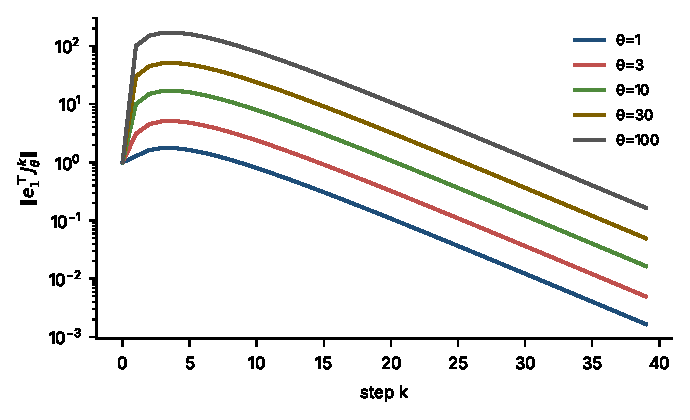
\includegraphics[width=0.6\textwidth]{figs/fig_blind.pdf}
\caption{Price-row transient gain of the spectral-blindness family $J_\theta$: eigenvalues $(0.8,0.7)$, one-step price variance 1 and stationary price variance 5 are the same for every $\theta$.}\label{fig:blind}
\end{figure}

Two clarifications prevent over-reading. First, the cohort economy of Section~\ref{sec:model} is itself non-normal, yet its price output does not amplify (Lemma~\ref{lem:cm}). Large weighted gains can be manufactured by output weights alone: with $C_w=(1,160)$, a price-and-memory functional peaks at $160.003$ at $t=0$, which is the static weight, not dynamic growth (Appendix~\ref{app:coordw}). Second, in a network of $M$ identical cohort economies coupled by symmetric nonnegative cross-impact, the coupled operator stays symmetric in the coordinates of Lemma~\ref{lem:cm}; with cross-impact $0.05$, the spectral radius rises from $0.822$ ($M=1$) to $0.973$ ($M=10$) while the Kreiss constant stays at one, as it must for a stable symmetric operator (\texttt{recompute\_oct20.py}). A stable normal contraction cannot exhibit Euclidean state-norm transient growth. This does not exclude scalar input-output overshoot relative to initial impact, which also depends on the input and output maps. The positive-cohort no-overshoot result is model-specific; the companion paper studies a depth-depletion mechanism.

